\documentclass[
  tucolor,
  BCOR=12mm,     % 12mm binding corrections, adjust to fit your binding
  parskip=half,  % new paragraphs start with half line vertical space
  open=any,      % chapters start on both odd and even pages
  cleardoublepage=plain,  % no header/footer on blank pages
]{tudothesis}


% Warning, if another latex run is needed
\usepackage[aux]{rerunfilecheck}

% just list chapters and sections in the toc, not subsections or smaller
\setcounter{tocdepth}{1}

%------------------------------------------------------------------------------
%------------------------------ Sprache und Schrift: --------------------------
%------------------------------------------------------------------------------
\usepackage{fontspec}
\defaultfontfeatures{Ligatures=TeX}  % -- becomes en-dash etc.

% german language
\usepackage{polyglossia}
\setdefaultlanguage{german}

% for english abstract and english titles in the toc
\setotherlanguages{english}

% intelligent quotation marks, language and nesting sensitive
\usepackage[autostyle]{csquotes}

% microtypographical features, makes the text look nicer on the small scale
\usepackage{microtype}

%------------------------------------------------------------------------------
%------------------------ Für die Matheumgebung--------------------------------
%------------------------------------------------------------------------------

\usepackage{amsmath}
\usepackage{amssymb}
\usepackage{mathtools}

% Enable Unicode-Math and follow the ISO-Standards for typesetting math
\usepackage[
  math-style=ISO,
  bold-style=ISO,
  sans-style=italic,
  nabla=upright,
  partial=upright,
]{unicode-math}
\setmathfont{Latin Modern Math}

% nice, small fracs for the text with \sfrac{}{}
\usepackage{xfrac}


%------------------------------------------------------------------------------
%---------------------------- Numbers and Units -------------------------------
%------------------------------------------------------------------------------

\usepackage[
  locale=DE,
  separate-uncertainty=true,
  per-mode=symbol-or-fraction,
]{siunitx}
\sisetup{math-micro=\text{µ},text-micro=µ}

%------------------------------------------------------------------------------
%-------------------------------- tables  -------------------------------------
%------------------------------------------------------------------------------

\usepackage{booktabs}       % stellt \toprule, \midrule, \bottomrule

%------------------------------------------------------------------------------
%-------------------------------- graphics -------------------------------------
%------------------------------------------------------------------------------

\usepackage{graphicx}
\usepackage{grffile}

% allow figures to be placed in the running text by default:
\usepackage{scrhack}
\usepackage{float}
\floatplacement{figure}{htbp}
\floatplacement{table}{htbp}

% keep figures and tables in the section
\usepackage[section, below]{placeins}

% package für feynman-grafen
\usepackage{tikz-feynman}

\usepackage{cancel}

%------------------------------------------------------------------------------
%---------------------- customize list environments ---------------------------
%------------------------------------------------------------------------------

\usepackage{enumitem}

%------------------------------------------------------------------------------
%------------------------------ Bibliographie ---------------------------------
%------------------------------------------------------------------------------

\usepackage[
  backend=biber,   % use modern biber backend
  autolang=hyphen, % load hyphenation rules for if language of bibentry is not
  sorting=none,    % german, has to be loaded with \setotherlanguages
                   % in the references.bib use langid={en} for english sources
]{biblatex}
\addbibresource{references.bib}  % die Bibliographie einbinden
\DefineBibliographyStrings{german}{andothers = {{et\,al\adddot}}}

%------------------------------------------------------------------------------
%------------------------------ Sonstiges: ------------------------------------
%------------------------------------------------------------------------------

\usepackage[pdfusetitle,unicode,linkbordercolor=tugreen]{hyperref}
\usepackage{bookmark}
\usepackage[shortcuts]{extdash}

% make bar horizontal, use \hslash for slashed h
\let\hbar\relax
\DeclareMathSymbol{\hbar}{\mathord}{AMSb}{"7E}
\DeclareMathSymbol{ℏ}{\mathord}{AMSb}{"7E}

% Self-made commands.
\newcommand{\upD}{\symup{\Delta}}
\newcommand{\upd}{\symup{d}}
\newcommand{\signal}{\symup{J}/\symup{\psi}\rightarrow e^{\pm}\mu^{\mp}}
\newcommand{\kontroll}{\symup{J}/\symup{\psi}\rightarrow \mu^{\pm}\mu^{\mp}}
\newcommand{\jpsi}{\symup{J}/\symup{\psi}}

%------------------------------------------------------------------------------
%-------------------------    Angaben zur Arbeit   ----------------------------
%------------------------------------------------------------------------------

\author{\vspace{3cm}\\Kevin Sedlaczek}
\title{\texorpdfstring{Suche nach dem Lepton-Flavor verletzenden Zerfall $\signal$ bei LHCb}{J/Psi to e µ}}
\subtitle{Normierungskonstante}
\date{2016}
\birthplace{Dortmund}
\chair{Lehrstuhl für Experimentelle Physik V}
\division{Fakultät Physik}
\thesisclass{Bachelor of Science}
\submissiondate{1. Juli 2016}
\firstcorrector{Dr.~Johannes Albrecht}
\secondcorrector{Prof.~Dr.~Bernhard Spaan}

% tu logo on top of the titlepage
\titlehead{
\includegraphics[height=1.5cm]{logos/tu-logo.pdf}}
\renewcommand*\chapterheadstartvskip{\vspace*{-0.2cm}}
\begin{document}
\frontmatter

\maketitle

% Gutachterseite
\makecorrectorpage

% hier beginnt der Vorspann, nummeriert in römischen Zahlen
\thispagestyle{plain}

\section*{Kurzfassung}
Diese Bachelorarbeit befasst sich mit der Bestimmung einer Normierungskonstante für den Zerfall $\signal$ über eine Analyse des Zerfalls $\kontroll$. Dazu wird auf im Jahre 2012 am LHCb-Detektor bei einer integrierten Luminosität von $\SI{2}{\femto\barn^{-1}}$ und einer Schwerpunkstenergie von $\SI{8}{\tera\electronvolt}$ aufgenommene Daten eine Selektion durchgeführt, aus welcher schließlich die Anzahl der Signalkandidaten bestimmt wird. Zusammen mit den während der Analyse bestimmten Effizienzen kann hieraus eine Normierungskonstante $\alpha$ berechnet werden. Der Zerfall $\signal$ ist im Standardmodell verboten, da er die Erhaltung des \textit{lepton-flavor} verletzt. Eine parallel durchgeführte Analyse beschäftigt sich mit der Optimierung der Suche nach Kandidaten für diesen Zerfall. Zusammen mit der Normierungskonstante kann eine obere Abschätzung für die Zerfallsbreite $\mathcal{B}(\signal)$ zu [blubb] bestimmt werden.

\section*{Abstract}
\begin{english}
This thesis aims at determining a normalisation factor $\alpha$ for the decay $\signal$, which is strictly forbidden within the standard model of particle physics, as it is violating the conservation of lepton-flavor. To achieve this, the similar decay $\kontroll$ is analysed. Within this analysis the selection of data taken in 2012 at the LHCb detector at a centre of mass energy of $\SI{8}{\tera\electronvolt}$, corresponding to an integrated luminosity of $\SI{2}{\femto\barn^{-1}}$ is optimized, so that a number of expected signal-events can be determined. Taking this number and the efficiencies of the selection into consideration, a normalisation factor is calculated. A simultaneously implemented study aims at the optimization of the search for $\signal$ events. Combining these two studies, an upper limit of [blubb] can be set for the branching fraction $\mathcal{B}(\signal)$.
\end{english}

\tableofcontents

\mainmatter
% Hier beginnt der Inhalt mit Seite 1 in arabischen Ziffern
\chapter{Einleitung}
%
Die Teilchenphysik beschäftigt sich mit dem Verständnis der Physik auf elementarster Ebene. Dazu gehört die Beschreibung der Elementarteilchen sowie deren Wechselwirkungen untereinander. Über die letzten Jahrzehnte ist dabei das sogenannte Standardmodell der Teilchenphysik entstanden, welches bis heute die beste Beschreibung in dieser Hinsicht liefert. Dennoch existieren Phänomene, die sich durch das Standardmodell nicht beschreiben lassen: die Existenz von dunkler Materie, Gravitation oder Neutrinooszillationen sind Beispiele dafür. Die ständige Überprüfung der Vorhersagen, sowie die Suche nach Physik, die über das Standardmodell hinaus geht sind Aufgaben von Physikern an Teilchenbeschleunigern wie dem LHC (Large Hadron Collider) der Europäischen Organisation für Kernforschung am CERN. \\
Eine parallel durchgeführte Untersuchung beschäfigt sich mit der Suche nach dem \textit{lepon-flavor}-verletzenden (LFV) Zerfall $\signal$, also Physik jenseits des Standardmodells \cite{ba-maik}. Um die Ergebnisse dieser Signalanalyse statistisch sicher physikalisch interpretieren zu können, beschäftigt sich diese Arbeit mit der Untersuchung und Analyse eines Kontrollkanals: $\kontroll$.
Dazu werden im Jahre 2012 am LHCb Experiment bei einer Luminosität von $\SI{2}{\femto\barn^{-1}}$ und einer schwerpunktsenergie von $\SI{8}{\tera\electronvolt}$ gemessene Daten analysiert. Da der Kontrollkanal ein im SM erlaubter, gut vermessener Prozess mit großem Verzweigungsverhältnis (hohe statistische Genauigkeit) ist, lassen sich hierfür in statistischer und messungsbedingter Ungenauigkeit deutlich verringerte Aussagen treffen. Die Normierungskonstante dient in der Analyse des Signalkanals der Abschätzung eines oberen Limits für die Zerfallsbreite des LFV Zerfalls. Zur Bestimmung dieser Variable werden die Daten für $\kontroll$ selektiert und analysiert.\\
Die Struktur dieser Arbeit ist viergeteilt: Zunächst wird in Kapitel~\ref{chap:2} das zugrundeliegende Standardmodell der Teilchenphysik, sowie der physikalische Hintergrund des betrachteten Zerfalls beschrieben. Kapitel~\ref{chap:3} beschäftigt sich mit der Konstruktion und Funktion des LHC und des LHCb Detektors. Es wird erläuert über welche Detektoren die verwendeten Datensätze erstellt werden. Der Hauptteil der Arbeit - die Analyse - wird in Kapitel~\ref{chap:4} behandelt. Dazu wird die parallel vorgenommene Analyse des Signalkanals $\signal$ kurz erläutert und anschließend die Ermittlung der Normierungskonstante vorgenommen. In einem letzten Schritt werden die beiden Ergebnisse kombiniert und eine obere Abschätzung für die Zerfallsbreite des Signalkanals bestimmt (Kapitel~\ref{chap:5}).

\chapter{Physikalischer Hintergrund}
\label{chap:2}
%
\section{Das Standardmodell der Teilchenphysik}
%
Das Standardmodell (SM) der Teilchenphysik beschreibt den Aufbau der Materie, sowie ihre Wechselwirkung auf elementarer Ebene. Sie stellt eine über viele Jahrzehnte auf der speziellen Relativitätstheorie sowie der Quantentheorie erwachsene und vielfältig getestete Theorie dar. Allgemein werden zunächst zwei Arten von Teilchen unterschieden: Fermionen (halbzahliger Spin $s=\sfrac{1}{2}$) und Bosonen (ganzzaliger Spin $s=1$). Die Fermionen im Standardmodell sind in drei Generationen von Quarks, sowie drei Generationen von Leptonen unterteilt, wie sie in Abbildng~\ref{fig:particles} aufgeführt sind. Die Leptonengenerationen bestehen hierbei aus einem ganzzahlig (in Einheiten der Elementarladung) geladenen punktförmigen Lepton ($e$, $\mu$, $\tau$), sowie den dazugehörigen ungeladenen und masselosen Neutrinos $\nu_e$, $\nu_\mu$, $\nu_\tau$.
%
\begin{figure}
  \centering
      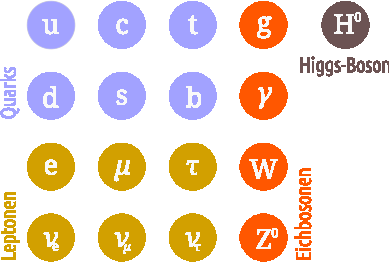
\includegraphics[width=0.6\textwidth]{Plots/SM.pdf}
  \caption{Die Elementarteilchen im Stadardmodell der Teilchenphysik.}
  \label{fig:particles}
\end{figure}
%
Auch die Quarks gliedern sich in drei Generationen. Diese erfolgt über die Eigenschaften der Teilchen: die Quarks lassen sich in \textit{up-artige} Quarks mit Ladung $\sfrac{2}{3}$, sowie \textit{down-artige} mit Ladung $\sfrac{-1}{3}$ einteilen. Es gilt für die Darstellung in Abbildung~\ref{fig:particles} dass die Teilchenmassen zwischen den Generationen von links nach rechts zunehmen.\\
Im Standardmodell unterscheidet man zwischen drei Wechselwirkungen der Elementarteilchen untereinander: die starke Wechselwrikung zwischen farbgeladenen Teilchen, die schwache Wechselwirkung an welcher alle Elementarteilchen teilnehmen, sowie die elektromagetische Wechselwirkung, welcher nur elektrisch geladene Teilchen unterliegen. Die letzten beiden lassen sich im Rahmen des SM zur elektroschwachen Wechselwirkung vereinigen.
Die Farbladung in der starken Wechselwirkung beschreibt das Konzept einer Quantenzahl deren Existenz zur theoretischen Umsetzung des sogenannten \textit{confinement} dient. \textit{confinement} meint hierbei die Tatsache, dass alle elementaren Teilnehmer der starken Wechselwirkung nur in "farbneutralen" (z.B. Farbe + Antifarbe) Zuständen frei existieren; freie Quarks lassen sich, da sie eine von null verschiedene Farbladung tragen also nicht beobachten.\\
%
Die Übertragung der Wechselwirkungen findet über die in Abbildung~\ref{fig:particles} genannten Bosonen statt. Bei der starken Wechselwirkung sind dies die Gluonen ($g$). Sie tragen eine Farbladung und einen ganzzahligen Spin $s=1$. Die Austauschteilchen der elektroschwachen Wechselwirkung sind die Photonen ($\gamma$) für den elektromagnetischen Teil, sowie für die schwache Wechselwirkung das neutrale $\symup{Z}$-Boson und die geladenen $\symup{W^{\pm}}$-Bosonen. \\
%
Aus den in Abbildung~\ref{fig:particles} aufgeführten Quarks (bis auf das \textit{top}-Quark) existieren über Kombination mehrere so genannte Hadronen - also aus Quarks zusammengesetzte Teilchen. Hierbei unterscheidet man die aus Quark und Antiquark bestehenden Mesonen und die aus drei Quarks (Antiquarks) bestehenden Baryonen. Zu den Mesonen zählt beispielsweise auch das $J/\!\symup{\psi}$ mit einem Quarkinhalt von $(c\bar{c})$, während das Proton ein prominenter Vertreter der Baryonen ist. Die meisten der aus den sechs Quarks sowie deren Antiteilchen gebildeten Hadronen sind nicht stabil, sodass sie über eine der oben genannten Wechselwirkungen in andere Hadronen sowie Leptonen zerfallen. Ähnliches lässt sich auch durch Streuprozesse oder Kollisionen erzielen, wie sie beispielsweise am LHC stattfinden.\\
%
Im Standardmodell sind bei all solchen Zerfällen diverse Erhaltungsgrößen zu beachten. Neben den klassischen Größen, wie etwa Energie- oder Impulserhaltung sind für die verschiedenen Wechselwirkungen auch einige Quantenzahlen im Teilchenzerfall invariant. Eines der fundamentalen Konzepte ist die \textit{lepton-flavor}-Erhaltung.
%
\section{\texorpdfstring{LFV und der Zerfall \signal}{Jpsi to eµ}}
%
Wie in der Einleitung bereits erwähnt, ist der Signalzerfall \signal ein im Standardmodell verbotener Zerfall, weil er die Erhaltung des \textit{lepton-flavor} verletzt. Jedem Lepton wird hierbei gemäß der in Abbildung~\ref{fig:particles} aufgeführten Generationen eine Quantenzahl zugeordnet (der \textit{lepton-flavor}). Elektronen oder Elektronneutrinos besitzen beispielsweise die Quantenzahl $l_e=1$, aber $l_\mu=0$, während Myonen $l_\mu=1$ und $l_e=0$ tragen. Antiteilchen wird jeweils der Wert $-1$ zugeordnet. So lassen sich Teilchenzerfälle auf die Erhaltung des \textit{lepton-flavor} überprüfen; der Zerfall \signal verstößt hierbei offensichtlich gegen diese Erhaltung.\\
%
Es gibt einige theoretische Vorhersagen über Mechanismen und Möglichkeiten der LFV; die meisten davon beschreiben Physik jenseits des Standardmodells. Ein im Standardmodell über Neutrinooszillation möglicher Zerfall ist in dem folgenden Feynmann-Diagramm dargestellt.
%
\begin{figure}[H]
  \centering
  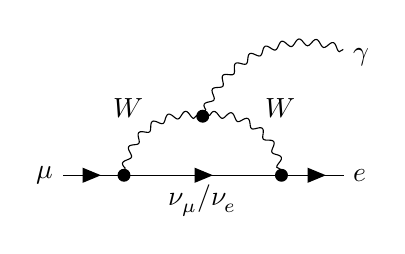
\begin{tikzpicture}
    \tikzfeynmanset{ every vertex={ black, dot}}
    \begin{feynman}
      \vertex (a1) {\(\mu\)};
      \vertex[right=1cm of a1] (a2);
      \vertex[right=2cm of a2] (a3);
      \vertex[right=1cm of a3] (a4) {\(e\)};
      \vertex at ($(a2)!1cm!(a3)!0.75!90:(a3)$) (d);
      \vertex[above=1.5cm of a4] (c){\(\gamma\)};
      \diagram*{
        (a1) -- [fermion](a2),
        %(a2) -- [fermion](a3),
        %(a2) -- [plain, edge label'=\(\nu_\mu\), insertion={0.5}] (a3),
        (a2) -- [fermion, edge label'=\(\nu_\mu/\nu_e\)](a3),
        (a2) -- [boson, quarter left, edge label=\(W\)] (d) [square dot] -- [boson,quarter left, edge label=\(W\)] (a3),
        (a3) -- [fermion](a4),
        (d) --  [photon, quarter left](c)
          };
    \end{feynman}
  \end{tikzpicture}
  \label{fig:lfv_nu}
\end{figure}
%
Da die Masse der Neutrinos nicht verschwindend ist, können so gennante Oszillationen in andere \textit{flavors} stattfinden. Über diesen Mechanismus ist ein Zerfall möglich der an jedem Vertex \textit{lepton-flavor}-erhaltend ist. Da die Massen der Neutrinos allerdings als sehr klein abgeschätzt werden können, sind die Beiträge dieses Zerfallskanals zu gering, als dass sie experimentell nachgewiesen werden können. Experimentelle Evidenz deutete daher auf Physik jenseits des Stadardmodells hin. Andere theoretische Beschreibungen gehen etwa von Zerfällen über ein $Z'$-Boson aus.\cite{zprime} Auch Prozesse über SUSY Teilchen sind nicht ausgeschlossen\cite{susy_gut1}\cite{susy_gut2}.

\chapter{Der Large Hadron Collider und der LHCb-Detektor}
\label{chap:3}
%
\section{Der Large Hadron Collider}
%
Der \textit{Large Hadron Collider} (LHC) \cite{lhc} am CERN ist der derzeit leistungsstärkste Teilchenbeschleuniger der Welt. Er dient der Erzeugung von Proton-Proton-Kollisionen ($pp$-Kollisionen), sowie weiteren Teilchenkollisionen bei einer Schwerpunktenergie von bis zu $\sqrt{s}=\SI{14}{\tera\electronvolt}$ \cite{lhc}. Diese durch Größe und Bauteile beschränkten Energien werden nach dem letzten Upgrade mit $\SI{13}{\tera\electronvolt}$ beinahe ausgereizt \cite{lhc}. Durch die Ausweitung des zu untersuchenden Energiebereiches auf diese Größenordnung eignet sich der LHC zur Entdeckung von Physik jenseits des SM, wie etwa unbekannter Teilchen. Im Jahre 2012 gelang der ATLAS- und der CMS-Kollaboration die Entdeckung des in den 60er-Jahren von Higgs, Englert und Brout vorhergesagten Higgs-Bosons \cite{higgs_atlas, higgs_cms}.\\
Bevor die Protonen im 50 bis $\SI{175}{\meter}$ \cite{lhc} unter der Erde liegenden, $\SI{27}{\kilo\meter}$ langen Speicherring auf die maximale Schwerpunktsenergie beschleunigt werden, durchlaufen sie ein vielschrittiges System aus Vorbeschleunigern. Dessen letzte Stufe ist der \textit{Super Proton Synchrotron} (SPS), welcher die Protonen auf etwa $\SI{99,99978}{\percent}$ der Lichtgeschwindigkeit beschleunigt \cite{lhc}. Diese Protonen werden mit einer Schwerpunktsenergie von $\SI{0,45}{\tera\electronvolt}$ über zwei Transferlinien in den LHC injiziert, wo sie in entgegengesetzter Richtung beschleunigt werden. Die Beschleunigung und Kreisführung findet dabei in einem Ultrahochvakuum über \textit{radio frequency}-Kavitäten und supraleitende Magnete, welche von flüssigem Helium auf etwa $\SI{1,9}{\kelvin}$ gekühlt werden, statt. So werden Hunderte einzelner Protonenbündel auf beinahe Lichtgeschwindigkeit beschleunigt und anschließend in Abständen von $\SI{25}{\nano\second}$
($\SI{40}{\mega\hertz}$) in einem der vier großen Experimente durch Strahlkreuzung zur Kollision gebracht. Da Datenmengen in dieser Größenordnung nicht gespeichert werden können, wird ein mehrstufiges Filtersystem angewendet: die Trigger. Diese sind in drei Stufen aufgeteilt. Der Hardwaretrigger \textsc{L0} trifft direkt bei der Messung in Echtzeit Entscheidungen, sodass die Ereignisrate ein prozessierbares Niveau ($\SI{1}{\mega\hertz}$) \cite{Tilburg} erreicht, gleichzeitig aber möglichst viele Ereignisse, die potenziell physikalisch relevant sind, aufgenommen werden. Dazu werden Daten aus den Kalorimetern, sowie den Myonkammern zur Bestimmung hoher Transversalimpulse bzw. Energien verwendet. Die Softwaretrigger (\textsc{HLT1} und \textsc{HLT2}) reduzieren kurz darauf die Datensätze auf physikalisch Relevantes. Der HLT1-Trigger führt dabei eine partielle Rekonstruktion der Events über Vertex- und Spurbestimmungen durch. Der HLT2-Trigger stellt die letzte Stufe dar und kann Entscheidungen auf Grundlage der gesamten Ereignis-Informationen treffen. So wird die Datenrate von $\SI{16}{\mega\hertz}$ auf etwa $\SI{2}{\kilo\hertz}$ reduziert.
%
\section{Der LHCb Detektor}
%
\begin{figure}[H]
  \centering
      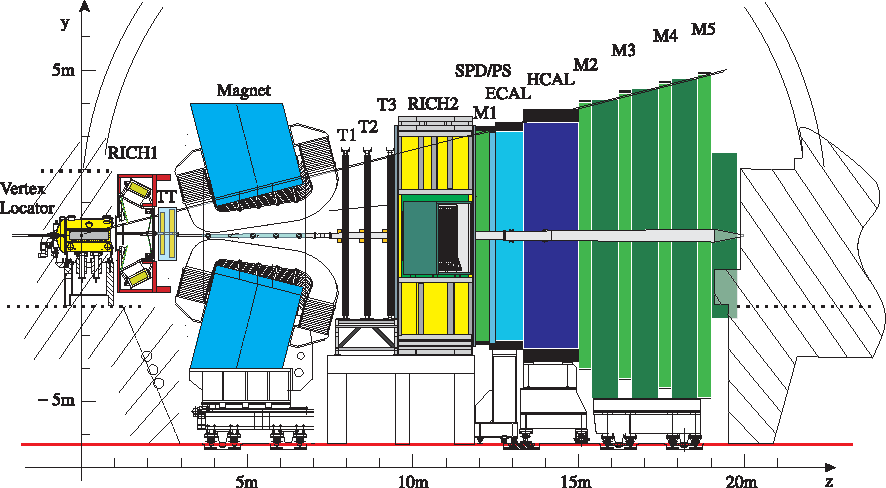
\includegraphics[width=0.89\textwidth]{Plots/lhcb.pdf}
  \caption{Querschnitt des LHCb-Detektors \cite{lhcb}.}
  \label{fig:lhcb}
\end{figure}
%
Der LHCb-Detektor deckt im Gegensatz zu den anderen drei Experimenten am LHC bei seinen Messungen nicht den gesamten Raumwinkel um den Kollisionspunkt ab. Es handelt sich hierbei um einen einarmigen vom Kollisionspunkt in einer der Strahlrichtungen vorwärtsgerichteten Detektor. Die Wahl dieser Bauart hängt unter anderem mit dem Hauptverwendungszweck des Detektors zusammen: Wie der Name schon impliziert ist die Untersuchung von $b$-Quarks bzw. B-Mesonen Hauptziel des Experimentes. Da sich diese nach ihrer Erzeugung in den $pp$-Kollisionen in Kegeln unter sehr kleinen Winkeln zum Protonstrahl bewegen, ist ein Detektor wie der LHCb auf die Vermessung dieses Bereiches optimal ausgelegt, da einer der beiden Zerfallskegel genau in den Detektor strahlt. Dieser Winkel in der Produktion der $B$-Mesonen ist dadurch begründet, dass der für die Erzeugung der B-Mesonen maßgebliche Prozess über Gluonen aus dem Quark-Gluon-Plasma abläuft. Diese Gluonen tragen kleine, asymmetrisch verteilte Impulsbruchteile, sodass die Impulse nach Kollision vergleichsweise stark in longitudinale Richtung weisen. Der Akzeptanzbereich des Detektors zur Strahlachse gemessen beträgt hierbei $10$\,mrad - $300$\,mrad. Dieser deckt bei einer Schwerpunktsenergie von $\SI{8}{\tera\electronvolt}$ etwa $\SI{27}{\percent}$ der $b$-Quarks ab \cite{rad}.\\
%
Der etwa $\SI{20}{\meter}$ lange Detektor ist aus mehreren Schichten verschiedener Detektoren und Messsysteme aufgebaut, die im Folgenden genauer erläutert werden. Dabei ist wenn von positiver z-Richtung die Rede ist, die Strahlrichtung vom Kollisionspunkt in den Detektor gemeint. Die Detektorsysteme lassen sich allgemein in zwei Arten von Detektoren unterteilen:
%
\begin{enumerate}
  \item Spurdetektoren: Vertex Locator (VELO), Tracker Turicensis (TT), Innerer Spurdetektor (IT), Äußerer Spurdetektor (OT)
  \item Teilchenidentifikation (PID): erster und zweiter Cherenkovdetektor (RICH 1 und RICH 2), elektromagnetisches und hadronisches Kalorimeter (ECAL und HCAL) sowie die Myondetektoren.
\end{enumerate}
%
Der dem Kollisionspunkt am nächsten liegende Detektor ist der \textbf{Vertex Locator}, kurz VELO. Seine Aufgabe ist die möglichst exakte Ermittlung der Zerfallsvertices, beispielsweise der B-Mesonen. Die in den Kollisionen entstehenden B-Mesonen zerfallen innerhalb von Strecken einiger Millimeter, weswegen die Detektoren unmittelbar um den Kollisionspunkt liegen, wenn Daten genommen werden \cite{Tilburg}. Da diese Region auch die am intensivsten von Strahlenschäden betroffene Region ist, ist der Detektor bei Injekion der Kollisionskandidaten mechanisch auf Abstand zu bringen.\\
Der VELO umgibt den Strahlrohr von zwei Seiten. Er besteht dabei im Einzelnen aus halbmondförmigen, $\SI{0.3}{\milli\meter}$ starken Scheiben von Spurdetektoren, die entlang des Strahlrohres angeordnet sind \cite{Tilburg}. Durchqueren geladene Teilchen die Siliziumscheiben, so erzeugen sie Elektron-Loch-Paare, welche elektronisch gemessen werden können und analog ausgelesen werden. Der während der Datennahme lediglich $\SI{7}{\milli\meter}$ vom Strahl entfernte VELO stellt neben dem TT den Hauptspurdetektor vor Einsatz des Magneten dar \cite{Tilburg}. \\
%
In der direkt vor dem Magneten liegenden von einem geringen Magnetfeld durchsetzten Region des Detektors befindet sich der \textbf{Tracker Turicensis}. Dieser zweigeteilte Detektor besteht aus zwei über insgesamt etwa $\SI{8.4}{\meter\squared}$ den gesamten Akzeptanzbereich des Detektors abdeckenden Silizium-Streifen-Detektoren \cite{lhcb}. Ihre Aufgabe ist die dreidimensionale Rekonstruktion von Teilchenspuren, sowie die Identifikation von neutralen Teilchen, deren Lebensdauern so groß sind, dass sie den VELO verlassen können (z.B. das $K_s^0$-Meson).\\
%
Das Spurbestimmungssystem T1-T3 besteht aus den \textbf{inneren Spurdetektoren} (IT), welche auf dieselbe Weise wie der TT arbeiten und den \textbf{äußeren Spurdetektoren} (OT) \cite{tracker}. Der IT bildet den direkt am Strahlrohr liegenden Teil der T-Tracker und zeigt damit das höchste Aufkommen an geladenen Teilchen. Sie führen wie die TT über einzelne Silizium-Detektormodule Spurmessungen mit einer Auflösung von etwa $\SI{50}{\micro\meter}$ durch \cite{Tilburg}. Diese Module sind in einem Bereich von $\SI{125}{\centi\meter}$ Weite und $\SI{40}{\centi\meter}$ Höhe kreuzförmig um das Strahlrohr ausgerichtet \cite{tracker}.\\
Die \textbf{äußeren Spurdetektoren} stellen den letzten Spurdetektor im LHCb dar. Sie decken den weitaus größeren Bereich der T1-T3 Spurdetektoren ab, der außerhalb der Akzeptanz der IT liegt; dabei übernehmen sie die gleiche Aufgabe, wie die Inneren Spurdetektoren.\\

Die Teilchenidentifikation (PID) erfolgt zunächst über zwei Cherenkov-Detektoren: das \textit{Ring Imaging Cherenkov} Detektor-System (\textbf{RICH}). Sie dienen vor Allem der Unterscheidung und Bestimmung vieler Hauptzerfallsprodukte der B-Mesonen \cite{lhcb}. Der erste dieser Detektoren (\textbf{RICH1}) befindet sich zwischen dem VELO und den T1-T3. Der zweite Detektor (\textbf{RICH2}) liegt nach dem letzten Tracking-System, (T3) aber noch vor den Kalorimetern (siehe Abbildung~\ref{fig:lhcb}). Cherenkov-Photonen entstehen, wenn sich ein geladenes Teilchen in einem Medium schneller bewegt, als sich Licht in Selbigem ausbreitet. Der Winkel unter dem diese Photonen abgestrahlt werden, ist abhängig von der Teilchengeschwindigkeit und dem Brechungsindex des Mediums. Daher kann aus diesem Winkel die Geschwindigkeit der Teilchen und zusammen mit dem Impuls die Masse dieser bestimmt werden. Diese Information lässt sich zur Identifikation der Teilchen nutzen. Die Auflösung der Detektoren liegt zwischen $2$ und $\SI{100}{\giga\electronvolt}$ \cite{lhcb}.\\
%
Bevor die Myonenkammern den Detektor abschließen, vermisst ein Kalorimetersystem die Energie der Teilchen. Dieses besteht aus einem elektromagnetischen Kalorimeter (\textbf{ECAL}) und einem hadronischen Kalorimeter (\textbf{HCAL}). In  diesen Kalorimetern werden alle Teilchen, bis auf Myonen, absorbiert. Dies geschieht über Wechselwirkungen mit dem Material, welche sogenannte Teilchenschauer erzeugen. Diese Schauer deponieren ihre Energie in Szintillatoren, indem sie diese anregen. Die daraufhin von den Szintillatoren emittierten Photonen können als Maß für die Energie der Teilchen gemessen werden. Die Energiebestimmung dient anschließend unter Anderem den Triggern dazu, Teilchen mit hoher transversaler Energie (also großer Impuls vom Strahlrohr weg) herauszufiltern \cite{lhcb}. Das ECAL misst dabei insbesondere die elektromagnetischen Schauer, die von Elektronen oder Photonen ausgelöst werden. Um die Teilchenidentifikation für das Kalorimeter zu verbessern befinden sich hier zwei weitere Detektoren vor dem ECAL. \\
Das HCAL fungiert wie das ECAL, vermisst dabei aber die von Hadronen (hauptsächlich Pionen, Kaonen und Protonen) ausgelösten Schauer. Es ist hinter dem ECAL positioniert. \\
%
Die \textbf{Myonenkammern} (\textbf{M1}-\textbf{M5} in Abbildung~\ref{fig:lhcb}) detektieren die den Detektor aufgrund ihres geringen Wirkunsgquerschnitts größtenteils ungestört durchquerenden Myonen. Sie bestehen aus auf fünf Detektorelemente aufgeteilte Vieldrahtproportionalkammern, in welchen die Impulse der Myonen und ihre Spuren gemessen werden. Das erste Detektorelement \textbf{M1} befindet sich dabei vor dem Kalorimetersystem und besitzt aufgrund des hohen Teilchenaufkommens sogenannte \textit{triple-GEM}-Folie \cite{Tilburg}. Nicht alle Myonen erreichen die Detektoren \textbf{M2}-\textbf{M5}, abhängig von ihren Impulsen. Diese befinden sich hinter dem Kalorimetersystem und decken die gesamte Akzeptanz des Detektors ab \cite{lhcb}.

\chapter{Analyse des Kontrollkanals}
\label{chap:4}
%
Ziel dieser Analyse ist es die benötigten Größen zur Bestimmung einer Normierungskonstante $\alpha$ für den Signalzerfall $\signal$ zu ermitteln. Diese ist in Gleichung~\eqref{eq:konst} definiert.
%
\begin{equation}
  \alpha=\frac{\mathcal{B}(B\rightarrow\jpsi K)\mathcal{B}(\kontroll)}{N_{\kontroll}}\frac{(\epsilon_{\text{ges}})_{\kontroll}}{(\epsilon_{\text{ges}})_{\signal}}
  \label{eq:konst}
\end{equation}
%

Hierbei ist~$\mathcal{B}(\kontroll)$ das bereits zu $\SI{5,986(33)}{\percent}$ \cite{pdg} vermessene Verzweigungsverhältnis des Kontrollkanals und~$N_{\kontroll}$ die in dieser Arbeit bestimmte Anzahl der gemessenen Signalereignisse für $B\rightarrow\jpsi(\rightarrow\mu\mu) K$.
$\epsilon_{\text{ges}}$ beschreibt die Gesamteffizienzen der Analyse des jeweiligen Kanals. Sie beinhalten die Detektion,
Rekonstruktion und Selektion der Ereignisse. Die Normierungskonstante ermöglicht es, systematische Fehler in der Bestimmung der
Signalkandidaten und Effizienzen des Signalzerfalls $\signal$ möglichst herauszukürzen und so ein deutlich exakteres Ergebnis
zu bestimmen. $\alpha$ kann dazu genutzt werden, zusammen mit der in \cite{ba-maik} ermittelten Anzahl erwarteter
Signalkandidaten eine Abschätzung für das Verzweigungsverhältnis des Zerfalls $\signal$ nach Gleichung~\eqref{eq:absch} zu ermitteln.
%
\begin{equation}
  \mathcal{B}(\signal)<N_{\signal, \SI{95}{\percent}}\cdot\alpha\, .
  \label{eq:absch}
\end{equation}
%
Ideal wäre die Betrachtung eines Datensatzes für $\kontroll$. Hierzu existiert allerdings bisher keine Vorselektion für Daten des LHCb, da sich diese noch in Vorbereitung befindet. Daher wird ein Datensatz für den Zerfall $B\rightarrow\jpsi(\rightarrow\mu\mu) K$ verwendet.
Da die Selektion für die darin enthaltenen Ereignisse aufgrund der Abweichung vom Signalzerfall ebenfalls abweichend ist, müssen bestimmte Korrekturen der erwarteten Ereignisse durchgeführt werden. Diese werden in Abschnitt~\ref{sec:norm} diskutiert.
Um die benötigten Größen aus dieser Analyse zu bestimmen, wird eine schnittbasierte Selektion des Kontrollkanals
durchgeführt, um über die Ermittlung der rekonstruierten Signalereignisse und der dabei auftretenden Effizienzen
die Normierungskonstante bestimmen zu können.
%
%%%%%%%%%%%%%%%%%%%%%%%%%%%%%%%%%%%%%%%%%%%%%%%%%%%%%%%%%%%%%%%%%%%%%%%%%%%%%%%%%%%%%%%%%%%%%%%%%%%%%%%%%%%%%%%%%%
\section{Datensätze}
%%%%%%%%%%%%%%%%%%%%%%%%%%%%%%%%%%%%%%%%%%%%%%%%%%%%%%%%%%%%%%%%%%%%%%%%%%%%%%%%%%%%%%%%%%%%%%%%%%%%%%%%%%%%%%%%%%
%
Bei dem für die Analyse des Zerfalls $\kontroll$ verwendeten Datensatz handelt es sich um im Jahre 2012 am LHCb-Experiment bei einer Schwerpunkstenergie von $\sqrt{s}=\SI{8}{\tera\electronvolt}$ aufgenommene Daten, die einer integrierten Luminosität von $\SI{2}{\femto\barn^{-1}}$ entsprechen. Dazu ist eine dem Zerfall $B^{+}\rightarrow\jpsi(\rightarrow\!\mu\mu) K^{+}$ angepasste Selektion (Stripping \texttt{Bu2LLK\_mmLine}) verwendet worden, welche eine Effizienz von $\SI{16,099(21)}{\percent}$ aufweist. Die Selektionsvariablen und die zugehörigen Kriterien sind in Tabelle~\ref{tab:bstrip} aufgeführt.
%
\begin{table}[htb]
  \centering
  \caption{Auf den Datensatz angewendete Selektion.}
  \begin{tabular}{lc}
    \toprule
    Selektionsvariable                & Bedingung      \\
    \midrule
    $m_{B}$                           & $>\num{5129}<\num{5429}$  \\
    $B^{+}:\chi_{\text{IP}}^2$        & $<\num{25}$  \\
    $B^{+}:\chi_{\text{VD,PV}}^2$     & $>\num{100}$  \\
    $B^{+}:\text{DIRA}$               & $>\num{0.9995}$  \\
    \bottomrule
  \end{tabular}
  \label{tab:bstrip}
\end{table}
%
Es wird also die rekonstruierte Masse des $B$-Mesons auf einen Bereich von $\pm\SI{150}{\mega\electronvolt}$ um die tatsächliche Masse von $\SI{5279.25(26)}{\mega\electronvolt}$ eingeschränkt. $\chi_{\text{IP}}^2$ ist dabei definiert als der Unterschied zwischen dem $\chi^2$ des Primärvertex' unter Berücksichtigung des beschriebenen Teilchens und jenem ohne Berücksichtigung desselben. Über $\chi_{\text{VD,PV}}^2$ wird die Flugdistanz des $B$-Mesons, die aufgrund seiner Lebensdauer entfernt vom Primärvertex liegt, nach unten beschränkt. Durch Wahl von Ereignissen mit $B^{+}:\text{DIRA}$ nahe $1$ werden solche selektiert, deren Winkel zwischen Impuls und rekonstruierter Spur des Teilchens möglichst gering und somit die Übereinstimmung möglichst groß ist.
Die verwendeten Daten enthalten dabei etwa 5959563 experimentell gemessene Daten, sowie etwa 2210052 in sogenannten Monte-Carlo-Simulationen generierte.\\

Monte-Carlo-Simulationen (MC) stellen eine bewährte Methode dar, um die Physik, die eine Theorie beschreibt und die experimentell gemessenen Daten vergleichbar zu machen. Um die Vorhersage für das Signal eines bestimmten Zerfalls in Form einer experimentellen Messung anzupassen, werden verschiedene Algorithmen zur Simulation der Kollisionen sowie deren Messung verwendet. Ziel ist es, die Kollision, anschließende Zerfälle sowie die Wechselwirkungen mit dem spezifischen Detektor möglichst exakt zu simulieren. So entsteht ein Signaldatensatz, welcher unter Anderem der Unterdrückung des experimentell gemessenen Untergrundes, sowie der Suche nach neuer Physik dient. Bei dem hier verwendeten MC handelt es sich um die Simulation des Zerfalls $B^{+}\rightarrow\jpsi(\rightarrow\!\mu\mu) K^{+}$. Dabei werden die Proton-Proton-Kollisionen durch das Programm \texttt{PYTHIA 8.1} \cite{pythia} simuliert, welches über komplexe Modelle die entstehenden Teilchen generiert. Zerfallspunkte sowie die Produkte der bei diesen Kollisionen entstehenden $B$-Mesonen werden durch \texttt{EVTGEN} \cite{evtgen} simuliert. Die anschließende Wechselwirkug der Zerfallsprodukte mit dem Detektor konstruiert der Algorithmus \texttt{GEANT4}  \cite{geant4}, sodass die so entstandenen Datensätze durch dieselbe Hardware und Software (Trigger, Rekonstruktion etc.), wie die experimentell am LHCb Gemessenen laufen können. Die Umwandlung der berechneten Ereignisse in die dazu benötigten elektrischen Signale übernimmt die Software \texttt{BOOLE} \cite{boole}. Die Simulation geht dabei von einer Schwerpunktsenergie von $\sqrt{s}=\SI{8}{\tera\electronvolt}$ aus. Um die Simulation den Beschaffenheiten des Detektors anzupassen, ist der Winkelbereich der Zerfallsprodukte auf einen etwas größeren als den realen Akzeptanzbereich des Detektors beschränkt. Hierdurch werden Effekte am Rand des Detektors vernachlässigbar.
%%%%%%%%%%%%%%%%%%%%%%%%%%%%%%%%%%%%%%%%%%%%%%%%%%%%%%%%%%%%%%%%%%%%%%%%%%%%%%%%%%%%%%%%%%%%%%%
\section{Selektion des Kontrollkanals}
%%%%%%%%%%%%%%%%%%%%%%%%%%%%%%%%%%%%%%%%%%%%%%%%%%%%%%%%%%%%%%%%%%%%%%%%%%%%%%%%%%%%%%%%%%%%%%%
Die Datensätze für den zu untersuchenden Kontrollkanal $B^{+}\rightarrow\jpsi(\rightarrow\mu\mu) K^{+}$ werden zunächst schnittbasiert selektiert. Es erfolgt also eine Einschränkung auf den physikalisch für den gesuchten Zerfall relevanten Bereich. Dazu werden die in Tabelle~\ref{tab:strip} aufgeführten Bedingungen an die relevanten Ereignisse in dem Datensatz sowohl an die Daten, als auch an die Simulation gestellt. Diese Selektion orientiert sich dabei an der in der Studie zur Signaloptimierung \cite{ba-maik} angewendeten.

\begin{table}[htb]
  \centering
  \caption{Auf den Datensatz angewendete Selektion.}
  \begin{tabular}{lc}
    \toprule
    Selektionsvariable                & Bedingung      \\
    \midrule
    $m_{\mu\mu}$                       & $>\num{2946}<\num{3176}$  \\
    $\mu^{-}:\chi_{\text{IP}}^2$      & $>\num{36}$  \\
    $\mu^{+}:\chi_{\text{IP}}^2$      & $>\num{36}$  \\
    $\mu^{-}:\text{GhostProb}$        & $<\num{0.3}$ \\
    $\mu^{+}:\text{GhostProb}$        & $<\num{0.3}$ \\
    $\jpsi:\text{BKGCAT}$(Nur MC)     & $==\num{0}$  \\
    $\jpsi:\text{DIRA}$               & $>\num{0}$  \\
    \bottomrule
  \end{tabular}
  \label{tab:strip}
\end{table}

Ziel dieser Selektion ist es, bei möglichst hoher Effizienz auf tatsächlich aus dem untersuchten Zerfall stammenden Ereignissen, möglichst viele Ereignisse aus sogenannten Untergrund-Zerfällen auszuschließen. Der bei allen Messungen unweigerlich in den Messungen dokumentierte Untergrund stellt eine Kombination verschiedener Teiluntergünde dar. Diese haben mitunter sehr unterschiedliche Ursachen. Der teilweise rekonstruierte Untergrund beispielsweise wird von Zerfällen induziert, die teilweise die selben Endprodukte wie der Signalzerfall erreichen, von denen allerdings nicht alle detektiert werden. Er überwiegt im unteren Massenfenster. Auch die Fehlerbehaftung der Messungen der einzelnen Detektorkomponenten erzeugt einen systematischen Untergrund, da die Messprozesse zwangsläufig statistischen Schwankungen unterliegen. Einen dritten Beitrag liefert der sogenannte kombinatorische Untergrund, der dadurch entsteht, dass beispielsweise zwei aus unabhängigen Zerfällen stammende Myonen, die zusammen zur Masse des $\jpsi$ kombiniert werden damit fälschlicherweise als Signal identifiziert werden.\\
Es wird zunächst ein Massenfenster von $m_{\mu\mu}=\SI{2946}{\mega\electronvolt}$ bis $m_{\mu\mu}=\SI{3176}{\mega\electronvolt}$ um die rekonstruierte Masse des $\jpsi$-Mesons von $\SI{3096.916(11)}{\mega\electronvolt}$ \cite{pdg} gelegt. Diese invariante Masse wird aus den Viererimpulsen der beiden Tochtermyonen berechnet, sodass durch das Fenster sichergestellt wird, dass diese auch aus einem $\jpsi$-Zerfall stammen. Die anderen Selektionsbedingungen sind aus einer rekursiven Optimierung des Signalzerfalls $\signal$ aus der parallel durchgeführten Studie \cite{ba-maik} übernommen, um eine optimale Vergleichbarkeit zu gewährleisten. Selbstverständlich sind sie für den Zerfall $\kontroll$ an die beiden Myonen angepasst.
Die Bedingungen $\mu^{\pm}:\chi_{\text{IP}}^2$ geben an, wie gut die rekonstruierten Myonen einem Primärvertex zugeordnet werden können. $\chi_{\text{IP}}^2$ ist dabei definiert als der Unterschied zwischen dem $\chi^2$ des Primärvertex' unter Berücksichtigung des beschriebenen
Teilchens und jenem ohne Berücksichtigung desselben \cite{chi2}. Die Variable $\mu^{\pm}:\text{GhostProb}$ gibt an, wie groß die Wahrscheinlichkeit
ist, dass die Identifikation eines Myons fälschlicherweise stattfand, sodass die Selektion diese Wahrscheinlichkeit auf maximal $\SI{30}{\percent}$
beschränkt. $\jpsi:\text{BKGCAT}$ legt fest, dass das in der Simulation rekonstruierte Ereignis auch als Signalereignis erzeugt wurde. Über die Variable $\jpsi:\text{DIRA}$ lässt sich die Übereinstimmung der Richtungen der aus den Vertices rekonstruierten Spuren sowie den Impulsen derselben Teilchen prüfen. Da es sich um den $cosinus$ des Winkels zwischen diesen Richtungen handelt, sollte diese Variable möglichst nahe bei $1$ liegen. Nach Anwenden der so gewählten Selektion auf die Simulation bleiben 1814293 Ereignisse. Die Effizienz dieser Selektion folgt daher nach Gleichung~\eqref{eq:eff_strip1}. Die Fehlerangaben entsprechen dabei den Binomial-Fehlern.
%
\begin{equation}
  \epsilon_\text{Selektion}=\frac{N_\text{MC-events after selection}}{N_\text{MC-events after strip}}=\SI{82.09(3)}{\percent} \, .%\frac{1814293}{2210052}
  \label{eq:eff_strip1}
\end{equation}
%
Des Weiteren werden sogenannte Triggerstufen als Bedingung für die Selektion der relevanten Ereignisse herangezogen. Die Trigger fungieren als Entscheidungskriterien dafür, ob ein Ereignis potentiell interessante Physik bereithält und somit vom Detektor aufgenommen und gespeichert werden soll, oder nicht. Die \texttt{TOS}-Trigger (\textit{triggered on signal}) lösen dabei aus, wenn Teilchen aus Signalzerfällen detektiert werden. Die hier, sowie in der Signalanalyse \cite{ba-maik} verwendeten Trigger gliedern sich in die in Tabelle~\ref{tab:trigger} aufgeführten drei Stufen \texttt{L0}, \texttt{HLT1} und \texttt{HLT2}. Diese sortieren nacheinander Ereignisse heraus, die nicht mindestens eine der aufgeführten Bedingungen innerhalb einer Stufe erfüllen. Daher selektiert jede Stufe feiner als die Vorherige.
%
\begin{table}[htb]
  \centering
  \caption{Auflistung der auf das $\jpsi$-Meson angewandten Trigger.
  Ereignisse, die nicht innerhalb jeder einzelnen Triggerstufe mindestens eine Triggerbedingung erfüllen, werden aussortiert.}
  \begin{tabular}{l}
    \toprule
    \textbf{L0-Trigger}                                 \\
    \quad\texttt{L0MuonDecision\_TOS}              \\
    \quad\texttt{L0HadronDecision\_TOS}            \\
    \quad\texttt{L0ElectronDecision\_TOS}          \\
    \midrule
    \textbf{HLT1-Trigger}                               \\
    \quad\texttt{Hlt1TrackAllL0Decision\_TOS}      \\
    \quad\texttt{Hlt1TrackMuonDecision\_TOS}       \\
    \midrule
    \textbf{HLT2-Trigger}                               \\
    \quad\texttt{Hlt2Topo2BodyBBDTDecision\_TOS}   \\
    \quad\texttt{Hlt2Topo3BodyBBDTDecision\_TOS}   \\
    \quad\texttt{Hlt2Topo4BodyBBDTDecision\_TOS}   \\
    \quad\texttt{Hlt2TopoMu2BodyBBDTDecision\_TOS} \\
    \quad\texttt{Hlt2TopoMu3BodyBBDTDecision\_TOS} \\
    \quad\texttt{Hlt2TopoMu4BodyBBDTDecision\_TOS} \\
    \bottomrule
  \end{tabular}
  \label{tab:trigger}
\end{table}
%
Die Effizienz $\epsilon$ dieser drei Triggerstufen, sowie desr Selektion bezogen auf die Zahl der Ereignisse im Datensatz beträgt für die Simulation die in Gleichung~\eqref{eq:eff_ges1} aufgeführten Wert.
%
\begin{equation}
  \epsilon_\text{Trigger}=\frac{N_\text{MC-events after trigger}}{N_\text{MC-events after selection}}=\SI{74.15(4)}{\percent} \, .% \frac{1345240}{1814293}
  \label{eq:eff_ges1}
\end{equation}
%
Zusammen mit der Generatoreffizienz $\epsilon_\text{gen}=\SI{16.099(21)}{\percent}$ und der Strippingeffizienz $\epsilon_\text{strip}=\SI{8.744(6)}{\percent}$ kann so die Gesamteffizienz wie in Gleichung~\eqref{eq:eff_ges} berechnet werden.
%
\begin{equation}
  \epsilon_{\kontroll, \text{ges}}
  =\epsilon_\text{gen}\cdot\epsilon_\text{strip}\cdot\epsilon_\text{Selektion}\cdot\epsilon_\text{Trigger}=\SI{0.857(1)}{\percent}
  \label{eq:eff_ges}
\end{equation}
%%%%%%%%%%%%%%%%%%%%%%%%%%%%%%%%%%%%%%%%%%%%%%%%%%%%%%%%%%%%%%%%%%%%%%%%%%%%%%%%%%%%%%%%%%%%%%%
\section{Massenfit}
%%%%%%%%%%%%%%%%%%%%%%%%%%%%%%%%%%%%%%%%%%%%%%%%%%%%%%%%%%%%%%%%%%%%%%%%%%%%%%%%%%%%%%%%%%%%%%%
Um aus dem so eingeschränkten und selektierten MC-Datensatz die Anzahl der Signalkandidaten $N_{\kontroll}$ zu bestimmen, wird ein sogennanter \textit{extended maximum-likelihood-fit} \cite{extended} der rekonstruierten $\jpsi$-Masse durchgeführt. Die oben
beschriebene Selektion beschränkt den Massenbereich des rekonstruierten $\jpsi$-Mesons auf einen Bereich von etwa
$[m_{\mu\mu}-\SI{150}{\mega\electronvolt}, m_{\mu\mu}+\SI{80}{\mega\electronvolt}]$. Die Masse des $\jpsi$-Mesons beträgt $\SI{3096.916(11)}{\mega\electronvolt}$ \cite{pdg}. Diese Einschränkung konzentriert den Fit auf die $\SI{60.87}{\percent}$ der gesamten Ereignisse, welche in diesem Bereich liegen, da so das gesamte Signal, aber möglichst wenig Untergrund vorliegen. Gleichzeitig ist das Intervall weit genug gewählt, um auch den eingangs dieses Kapitels beschriebenen Untergrund hinreichend modellieren zu können.
%
%\begin{figure}[H]
%  \centering
%      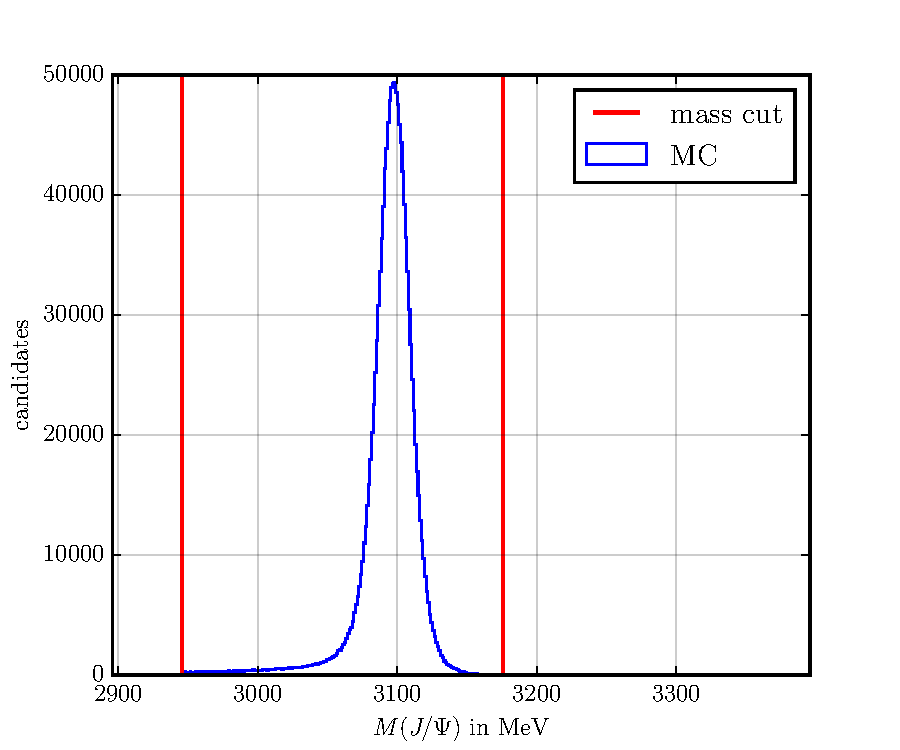
\includegraphics[width=0.9\textwidth]{Plots/jpsi_mass.pdf}
%  \caption{Verteilung der $\jpsi$-Masse nach Anwenden der Selektion sowie der Trigger.}
%  \label{fig:mass}
%\end{figure}
%
Mit Hilfe des frameworks \texttt{RooFit} \cite{roofit} wird diese Verteilung der rekonstruierten $\jpsi$-Masse an ein aus Signalmodell und Untergundmodell bestehendes Gesamtmodell angepasst. Dazu wird für ein aus Signalfunktion und Untergrundfunktion zusammengesetztes Modell der in Gleichung~\ref{eq:massenfit} dargestellten Form eine Ausgleichrechnung durchgeführt.
%
\begin{equation}
  \symup{G}(m_{\mu\mu})= \symup{S}(m_{\mu\mu}) + \symup{B}(m_{\mu\mu})
  \label{eq:massenfit}
\end{equation}
%
$\symup{S}(m_{\mu\mu})$ beschreibt hierbei das verwendete Signalmodell, während $\symup{B}(m_{\mu\mu})$ den Untergrund modelliert. Die Verteilung der Massen entspricht in etwa einer Gaußverteilung, zeigt aber an den Rändern sogenannte \textit{tails}: nicht der Normalverteilung entsprechende, beispielsweise durch Polynome beschriebende Verteilungen. Diese werden unter Anderem durch die Abstrahlung von niederenergetischen Photonen in Form von \textit{final state radiation} erzeugt \cite{cb}. Um diese Eigenschaft der Verteilung hinreichend zu modellieren, werden sogenannte \textit{Crystal Ball}-Funktionen (CB) verwendet. Diese zur Modellation asymmetrischer Wahrscheinlichkeitsverteilungen verwendeten Funktionen stellen eine Gaußfunktion dar, welche an einer Seite in eine Potenzfunktion übergeht. Die Darstellung ist in Gleichung~\ref{eq:cb} \cite{cb} angegeben, wobei die Parameter $A$ und $B$ stets so bestimmt werden, dass die Funktion analytisch ist.
%
\begin{equation}
  {\displaystyle CB(x;\alpha ,n,{\mu},\sigma,N)=N\cdot {\begin{cases}\exp \left(-{\frac {(x-{\mu})^{2}}{2\sigma ^{2}}}\right),&{\mbox{falls }}{\frac {x-{\mu}}{\sigma }}>-\alpha \\A\cdot \left(B-{\frac {x-{\mu}}{\sigma }}\right)^{-n},&{\mbox{falls }}{\frac {x-{\mu}}{\sigma }}\leqslant -\alpha \end{cases}}}
  \label{eq:cb}
\end{equation}
%
Als Modell für den Untergrund in dieser Messung wird ein exponentieller Zusammenhang der in Gleichung~\ref{eq:exp} dargestellten Form verwendet.
%
\begin{equation}
  B(x; c)= \symup{e}^{c\cdot x} \, .
  \label{eq:exp}
\end{equation}
%
Da durch nicht gaußverteilte Detektoreffekte \textit{tails} auch bei höheren Energien entstehen, kann es sinnvoll sein, durch die Kombination von zwei CB-Funktionen, also einem \textit{Double-Crystal-Ball} (DCB) die Modellation dieser zu ermöglichen \cite{ipatia}.
Im Folgenden wird der Signalteil der Verteilung der rekonstruierten Masse also als DCB-Funktion modelliert. Dies entspricht einem Gesamtmodell der in Gleichung~\ref{eq:dcb} dargestellten Form.
%
\begin{equation}
  \begin{split}
  \symup{G}(m_{\mu\mu}; f)={}&\symup{CB}_1(m_{\mu\mu};\alpha_1,\mu,\sigma_1,n_1) + f\symup{CB}_2(m_{\mu\mu};\alpha_2,\mu,\sigma_2,n_2)\\ &+ \symup{B}(m_{\mu\mu};c)
  \end{split}
  \label{eq:dcb}
\end{equation}
%
Der Faktor $f$ beschreibt dabei das Verhältnis der beiden CB-Funktionen und liegt zwischen 0 und 1. Zu dieser Funktion wird der oben beschriebene exponentielle Untergrund ($\symup{B}(m_{\mu\mu})$) hinzugefügt und das so entstehende Gesamtmodell an die Daten angepasst. Dazu werden die in Gleichung~\eqref{eq:dcb} aufgeführten Parameter mit Hilfe von \texttt{RooFit} der Verteilung angepasst.
%
%
%\begin{table}[H]
%  \centering
%  \caption{Auflistung der für den Fit des Signalmodells verwendeten Parameter.}
%  \begin{tabular}{ccc}
%    \toprule
%    \textbf{Crystall Ball 1}    & \textbf{Crystall Ball 2} & Intervall für den Fit \\
%    \midrule
%    $\alpha_1$                  & $\alpha_2$               & [-4, 0], [0, 4] \\
%    $\mu$                       & $\mu$                    & [2946, 3176] \\
%    $\sigma_1$                  & $\sigma_2$               & [1, 20], [1, 20] \\
%    $n_1$                       & $n_2$                    & [0, 20], [0, 20] \\
%    \bottomrule
%  \end{tabular}
%  \label{tab:params}
%\end{table}
%
$\alpha$ gibt dabei an, ab wann die Gaußverteilung durch den Potenzzusammenhang ersetzt wird. Dies beeinflusst also, wann die Modellation der \textit{tails}
einsetzt. Ein positives $\alpha$ bedeutet dabei, dass der \textit{tail} zu kleineren Werten einsetzt, während ein $\alpha<0$
diesen zu größeren Werten modelliert. $\mu$ beschreibt den Wert für das Maximum der Gaußfunktion. Anschaulich beschreibt dies die aus
den Daten rekonstruierte Masse des $\jpsi$-Mesons. Da beide \textit{Crystal Ball}-Funktionen an den gleichen Guaßschen Teil der Verteilung angepasst werden,
wird über diesen Parameter für beide Funktionen gemeinsam iteriert. Das $\sigma$ gibt wie bei Gaußschen Verteilungen üblich die Breite der Verteilung an. Über den Parameter $n$ kann das Modell für den \textit{tail} angepasst werden. Der Wert für $n$ gibt den Grad der Potenz an.
Die Ausgleichsrechnung ergibt die in Tabelle~\ref{tab:fit1} dargestellten Werte für die freien Parameter. Die so definierte Gesamtfunktion, sowie die einzelnen Komponenten sind in Abbildung~\ref{fig:fit1} dargestellt. Die Wahl mehrerer CB Funktionen ermöglicht es unter anderem, die Gaußverteilung, also den Kern des Fits zu verzerren. Auf diese Weise, ist das Gesamtmodell in der Lage auch nicht gaußverteilte Unsicherheiten in diesem Bereich zu modellieren. Allerdings ist die Ausgleichsrechnung mit \texttt{RooFit} für Modelle dieser Art numerisch sehr instabil, sodass die Wahl der Intervalle und Startwerte für die freien Parameter großen Einfluss auf das Ergebnis hat. Daher ist eine systematische und zuvor genau zu untersuchende Bestimmung dieser von Nöten, welche über den in dieser Arbeit gesteckten Rahmen hinaus ginge. [Was zu Ergebnissen, Fehlern etc...]
%
\begin{table}[H]
  \centering
  \caption{Auflistung der Fit-Ergebnisse des Signalmodells (DCB), sowie des exponentiellen Hintergrunds.}
  \begin{tabular}{lS@{$\,\pm$}S}
    \toprule
    \textbf{Signalmodell}         &  \multicolumn{2}{c}{Fit-Ergebnis} \\
    \midrule
    \quad$\alpha_1$               & 1,41    & 0,04 \\
    \quad$\mu$                    & 3097,79 & 0,02 \\
    \quad$\sigma_1$               & 10,08   & 0,09 \\
    \quad$n_1$                    & 1,49    & 0,07 \\
    \quad$\alpha_2$               & -1,54   & 0,04 \\
    \quad$\mu$                    & 3097,79 & 0,02 \\
    \quad$\sigma_2$               & 13,4    & 0,2 \\
    \quad$n_2$                    & 89      & 50 \\
    \quad$f$                      & 0,52    & 0,01 \\
    \quad$n_{BKG}$                & 4490    & 1394 \\
    \quad$n_{Sig}$                & 1342070 & 1175 \\
    \midrule
    \textbf{Untergrundmodell}     &  \multicolumn{2}{c}{Fit-Ergebnis} \\
    \midrule
    \quad$c$                      & -0,008   & 0,002 \\
    \bottomrule
  \end{tabular}
  \label{tab:fit1}
\end{table}
%
\begin{figure}[H]
  \centering
      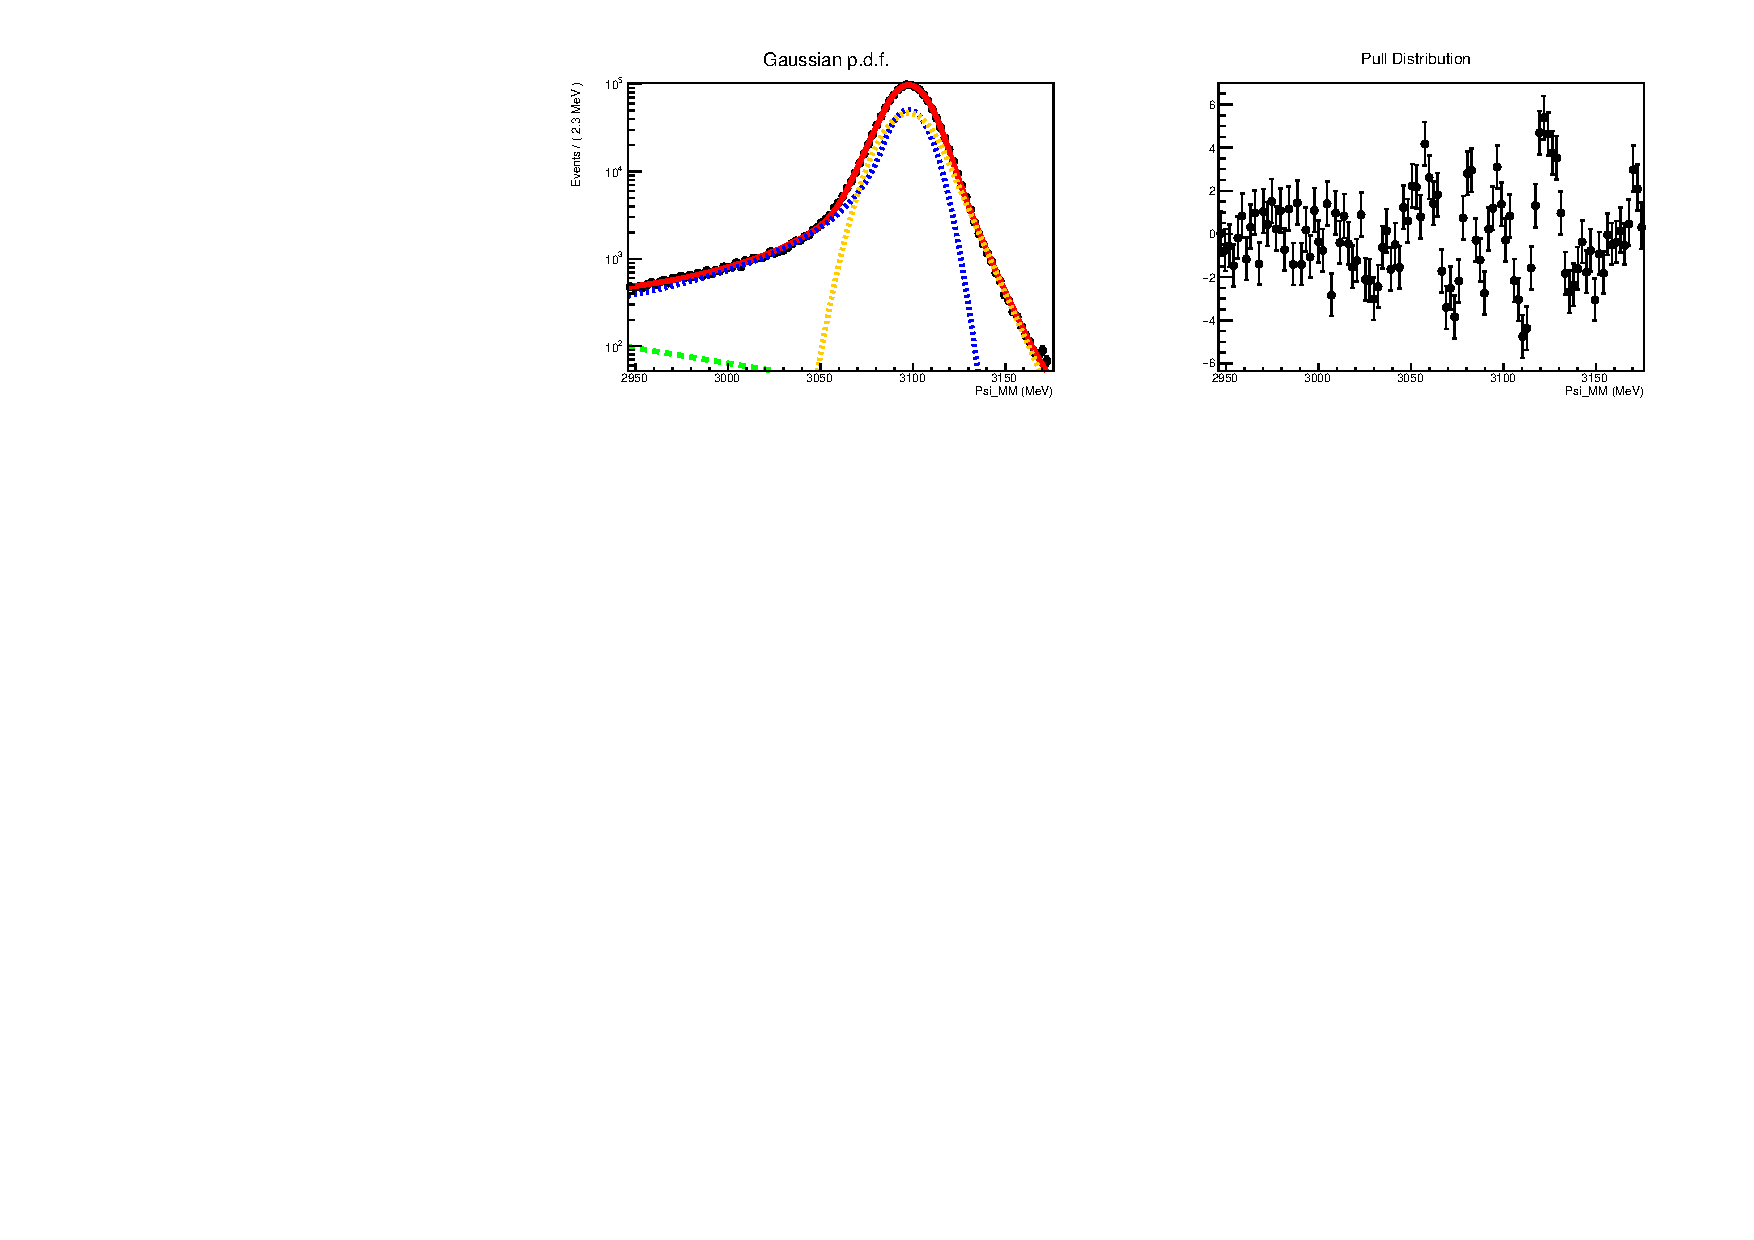
\includegraphics[width=1.2\textwidth]{Plots/DCBexp.pdf}
  \caption{Hier kommt eine Verteilung der $\jpsi$-Masse sowie das Ergebnis des DCB Fits in dieser Art (schöner vor endgültiger Abgabe) hin (grün: Untergrund, rot: Gesamtmodell, blau: CB1, orange: CB2).}
  \label{fig:fit1}
\end{figure}
%
%%%%%%%%%%%%%%%%%%%%%%%%%%%%%%%%%%%%%%%%%%%%%%%%%%  IPATIA  %%%%%%%%%%%%%%%%%%%%%%%%%%%%%%%%%%%%%%%%%%%%%%%%%%%%%%%%%%%%%%
Um der oben beschriebenen numerischen Instabilität vorzubeugen, kann beispielsweise die sogenannte IPATIA-Funktion als Signalmodell verwendet werden. Diese ist in Referenz~\cite{ipatia} genau beschrieben. Das ihr zugrunde liegende Modell berücksichtigt die oben erwähnten \textit{tails} und ermöglicht die Verzerrung der gaußschen 'Kernverteilung'. Dazu wird  ein Gesamtmodell der in Gleichung~\ref{eq:ipatia} dargestellten Form verwendet.
%
\begin{equation}
  \begin{split}
  &\symup{I}(m,\mu,\sigma,\lambda,\zeta,\beta,a,n)\propto\\
    &\begin{cases}
      \begin{split}
      ((m-\mu)^2&+A_\lambda²(\zeta)\sigma²)^{\frac{1}{2}\lambda-\frac{1}{4}}\symup{e}^{\beta(m-\mu)}\\
      &\cdot K_{\lambda-\frac{1}{2}}\left(\zeta\sqrt{1+(\frac{m-\ mu}{A_\lambda(\zeta)\sigma})^2}\right),
      \end{split} & \text{wenn} \frac{m-\mu}{\sigma}>-a \\
      \frac{G(\mu-a\sigma,\mu,\sigma,\lambda,\zeta,\beta)}{\left(1-m\/(n\frac{G(\mu-a\sigma,\mu,\sigma,\lambda,\zeta,\beta)}{G'(\mu-a\sigma,\mu,\sigma,\lambda,\zeta,\beta)}-a\sigma)\right)^n} ,& \text{sonst}
    \end{cases}
  \end{split}
  \label{eq:ipatia}
\end{equation}
%
Die Funktion $G(\mu-a\sigma,\mu,\sigma,\lambda,\zeta,\beta)$ ist dabei der für $\frac{m-\mu}{\sigma}>-a$ definierte Zusammenhang. Bei $K$
handelt es sich um Bessel-Funktionen dritter Gattung. $A_\lambda$ steht der Übersichtlichkeit halber als Abkürzung für
%
\begin{align*}
  A_\lambda^2=\frac{\zeta K_\lambda(\zeta)}{K_{\lambda+1}(\zeta)}\; .
\end{align*}
%
Das Signalmodell wird über die insgesamt neun, in Gleichung~\eqref{eq:ipatia} aufgeführten Parameter an die Massenverteilung angepasst.\\
Die Ausgleichsrechnung ergibt die in Tabelle~\ref{tab:fit2} dargestellten Parameter. Die so definierte Gesamtfunktion, sowie die einzelnen Komponenten sind in Abbildung~\ref{fig:fit2} dargestellt. [Fit ist bisher noch nicht konvergiert. Ergebnisse, Fehler etc...]
%
\begin{table}[H]
  \centering
  \caption{Auflistung der Fit-Ergebnisse des Signalmodells (IPATIA), sowie des exponentiellen Hintergrunds.}
  \begin{tabular}{lS@{$\,\pm$}S}
    \toprule
    \textbf{Signalmodell}         &  \multicolumn{2}{c}{Fit-Ergebnis} \\
    \midrule
    \quad$a$                      & 2,4      & 0,02 \\
    \quad$a_2$                    & 4,0      & 0,1  \\
    \quad$n$                      & 1,27     & 0,02 \\
    \quad$n_2$                    & 7,00     & 0,1 \\
    \quad$\beta$                  & -0.0136  & 0,0002 \\
    \quad$\zeta$                  & 0        & 0 \\
    \quad$\lambda$                & -2.5     & 0 \\
    \quad$\sigma$                 & 0,15     & 0,01 \\
    \quad$n_\text{BKG}$           & 8000     & 27 \\
    \quad$n_\text{Sig}$           & 1337610  & 1066 \\
    \midrule
    \textbf{Untergrundmodell}     &  \multicolumn{2}{c}{Fit-Ergebnis} \\
    \midrule
    \quad$c$                      & -0,0093   & 0,0005 \\
    \bottomrule
  \end{tabular}
  \label{tab:fit2}
\end{table}
%
\begin{figure}[H]
  \centering
      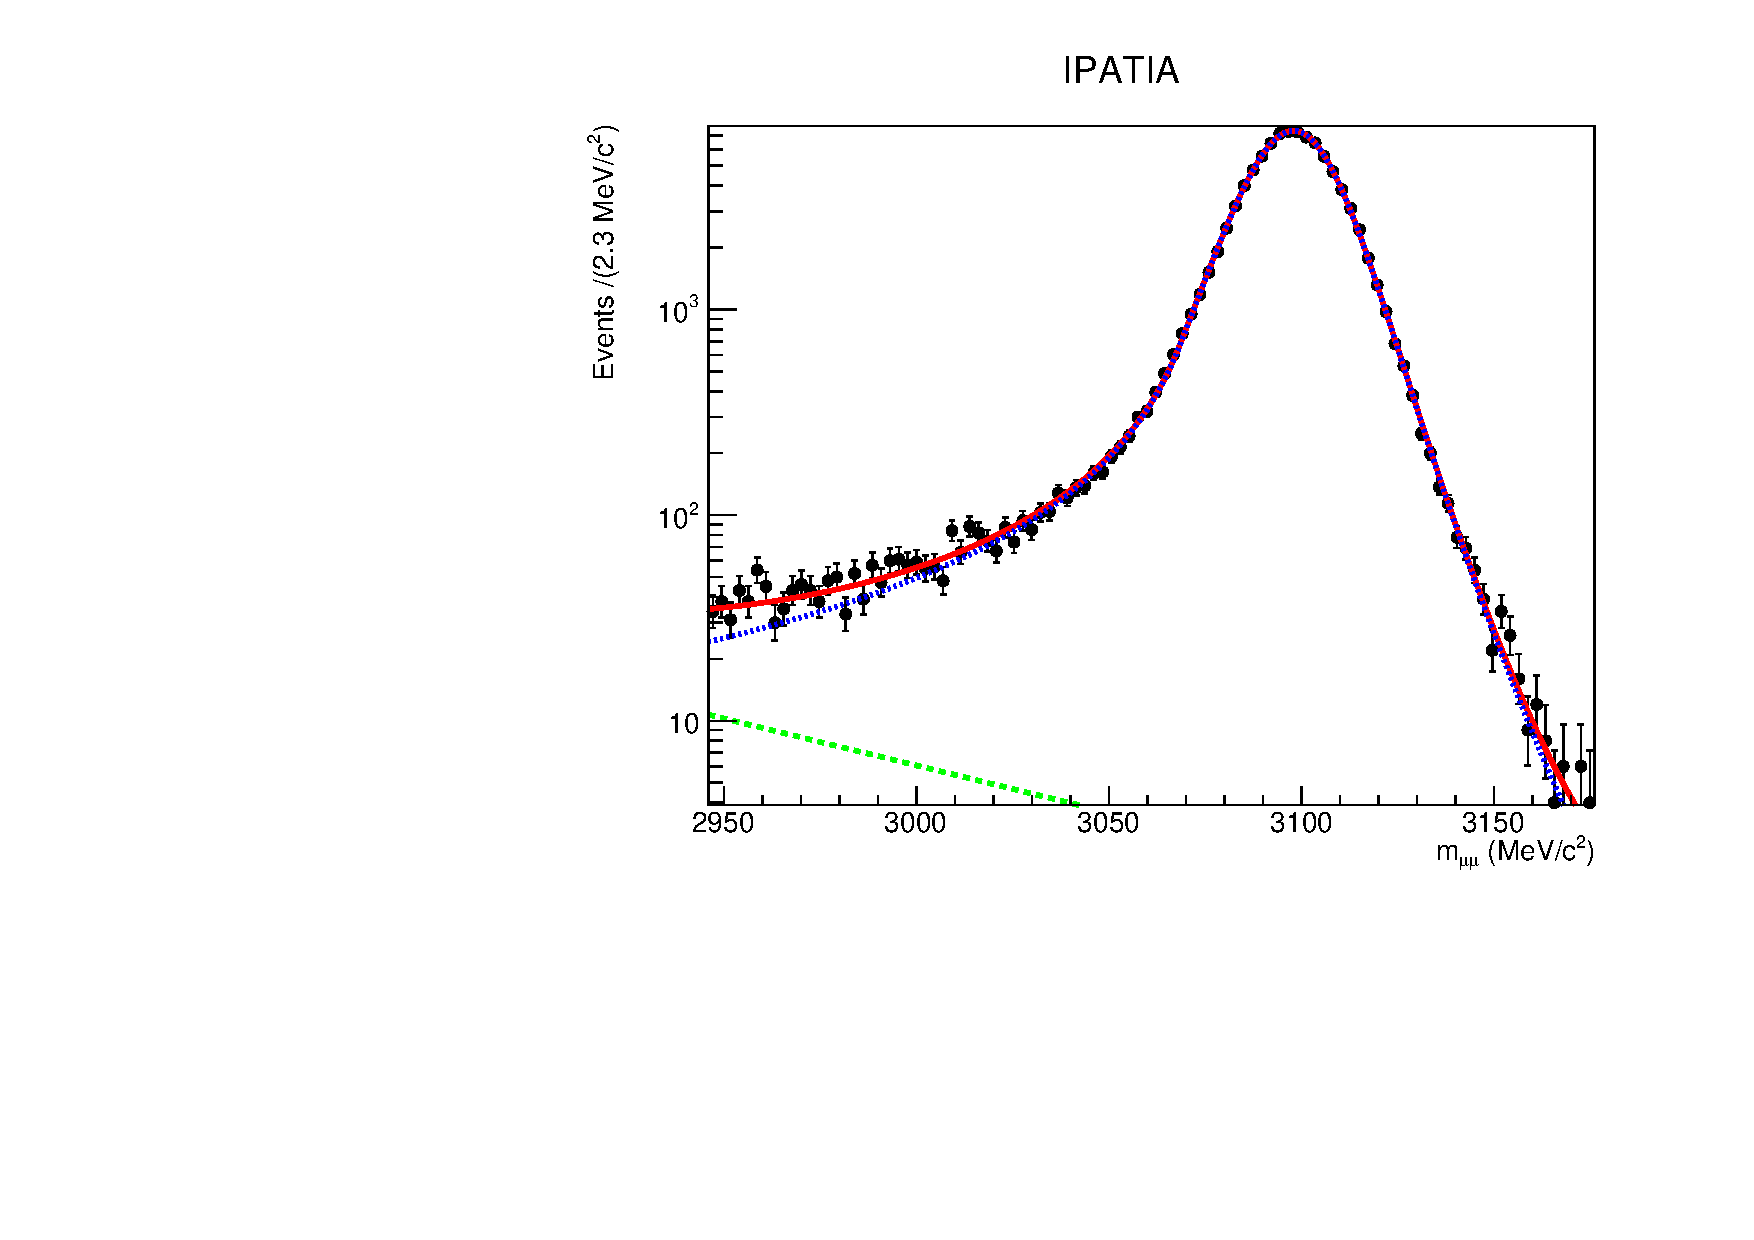
\includegraphics[width=\textwidth]{Plots/IPATIAexp.pdf}
  \caption{Hier kommt eine Verteilung der $\jpsi$-Masse sowie das Ergebnis des IPATIA Fits in dieser Art (schöner und mit Legende vor endgültiger Abgabe) hin (grün: Untergrund, rot: Gesamtmodell, blau: IPATIA).}
  \label{fig:fit2}
\end{figure}
%%%%%%%%%%%%%%%%%%%%%%%%%%%%%%%%%%%%%%%%%%%%%%%%%%%%%%%%%%%%%%%%%%%%%%%%%%%%%%%%%%%%%%%%%%%%%%%
\section{Bestimmung der Signalkandidaten}
%%%%%%%%%%%%%%%%%%%%%%%%%%%%%%%%%%%%%%%%%%%%%%%%%%%%%%%%%%%%%%%%%%%%%%%%%%%%%%%%%%%%%%%%%%%%%%%
Aus den oben durchgeführten Ausgleichsrechnungen folgt, dass sich die Anzahl der Signalkandidaten für $\kontroll$ am exaktesten über das Signalmodell \textsc{IPATIA} bestimmen lässt. Die Anzahl der Signalkandidaten folgt hierbei aus der Ausgleichsrechnung zu: $N_{\kontroll}=1337610\,\pm\,1066$ (Auf Fehler runden?) [wird ergänzt].
Kann auch über $N_{erw}=\mathcal{L}\cdot 2\sigma_{b\bar{b}}\cdot\mathcal{B}(\kontroll)\cdot\epsilon_{\kontroll, ges}$ berechnet werden, aber abhängig von der Genauigkeit der Lumi und des $\sigma_{b\bar{b}}$...
%%%%%%%%%%%%%%%%%%%%%%%%%%%%%%%%%%%%%%%%%%%%%%%%%%%%%%%%%%%%%%%%%%%%%%%%%%%%%%%%%%%%%%%%%%%%%%%
\section{Bestimmung der Normierungskonstante}
\label{sec:norm}
%%%%%%%%%%%%%%%%%%%%%%%%%%%%%%%%%%%%%%%%%%%%%%%%%%%%%%%%%%%%%%%%%%%%%%%%%%%%%%%%%%%%%%%%%%%%%%%
Aus der parallel durchgeführten Analyse \cite{ba-maik} wird die Gesamteffizienz für die Bestimmung der Signalkandidaten zu
%
\begin{equation}
  \epsilon_{\signal, \text{tot}}=1,2\,\pm\,0,4\cdot 10^{-6}
\end{equation}
%
referenziert. Das Verzweigungsverhältnis für den Zerfall $\kontroll$ ist zu \\$\SI{5,961(33)}{\percent}$ bestimmt \cite{pdg}. Der in
dieser Analyse verwendete Datensatz unterscheidet sich von dem in der Analyse \cite{ba-maik} verwendeten in der Vorselektion. Die
Kandidaten für den Zerfall $\kontroll$ werden so selektiert, dass die Impulse der beiden Myonen die Masse des $\jpsi$-Mesons
rekonstruieren und dass das $\jpsi$-Meson zusammen mit dem $K^+$ aus dem Zerfall eines $B$-Mesons stammt. Für die Selektion der Kandidaten für $\signal$ werden zwar auch Elektron-Myon-Paare gesucht, deren Impulse die Masse des $\jpsi$-Mesons rekonstruieren, allerdings wird
hier nicht die Rekonstruktion zu einem $B$-Meson vorgenommen. Sie wird dadurch ersetzt, dass der Zerfallsvertex der Myonen nicht direkt
am Kollisionspunkt liegen darf. Da dieser Unterschied Einfluss auf die Zahl der Signalkandidaten hat, bedarf es einer Korrektur. Eine Korrektur der Anzahl der ermittelten Signalkandidaten kann über den in Gleichung~\eqref{eq:korrektur} definierten Zusammenhang mit Hilfe des Faktors $R$ erfolgen.
%
\begin{equation}
  N_{\kontroll,\text{korr}}=N_{\kontroll}\cdot\underbrace{\frac{\sigma(pp\rightarrow\jpsi)}{\sigma(pp\rightarrow B^+)}}_{R}
  \label{eq:korrektur}
\end{equation}
%
Das Verhältnis aus $\sigma(pp\rightarrow\jpsi)$ und $\sigma(pp\rightarrow B^+)$ spiegelt hierbei ein Maß für die
Produktionswahrscheinlichkeit der beiden Mesonen wider. Dadurch wird die zusätzliche Beschränkung der $\kontroll$-Kandidaten auf die Herkunft aus einem B-Zerfall ausgeglichen. Der Wirkungsquerschnitt $\sigma(pp\rightarrow\jpsi)$ ist dabei Messungen der LHCb Kollaboration entnommen \cite{sigmajpsi}; der Wirkungsquerschnitt $\sigma(pp\rightarrow B^+)$ entspricht dem in \cite{sigmaB} gemessenen und ist zusätzlich über einen Faktor von $\sfrac{8}{7}$ auf die Schwerpunktsenergie von $\SI{8}{\tera\electronvolt}$ skaliert. \\ Der Korrekturfaktor berechnet sich gemäß Gleichung~\eqref{eq:korrfaktor}.
%
\begin{equation}
  R=\frac{\sigma(pp\rightarrow\jpsi)}{\sigma(pp\rightarrow B^+)}=\frac{\SI{1.14(16)}{\micro\barn}}{\SI{44.46(324)}{\micro\barn}}=???\,\pm\,???
  \label{eq:korrfaktor}
\end{equation}
%
Die so korrigierte Zahl an Signalereignissen entspricht
%
\begin{equation}
  N_{\kontroll,\text{korr}}=???\,\pm\,???\; .
\end{equation}
%
Da die bei dieser Korrektur verwendeten Wirkungsquerschnitte mit nicht zu vernachlässigenden Fehlern behaftet sind, kann
zum vergleich des Ergebisses der Korrekturfaktor über eine weitere Methode bestimmt werden. Dazu wird zunächst über die in
dieser Arbeit bestimmte Anzahl an $\kontroll$ Zerfällen auf die Zahl der insgesamt detektierten $B^{+}$-Mesonen zurückgerechnet. Über das Verhältnis der Produktionsrate des $B^{+}$- und des $B^{0}$-Mesons folgt damit die Zahl der
$B$-Mesonen[...]. Aus diesem Wert lässt sich dann über das Verzweigungsverhältnis für den Zerfall in $\jpsi$-Mesonen die korrigierte Zahl der Signalkandidaten bestimmen. Diese entspricht dem in Gleichung~\eqref{eq:korrfaktor2} definierten Wert.
%
\begin{equation}
  N_{\kontroll,\text{korr}}=\frac{N_{\kontroll}}{\mathcal{B}(B\rightarrow\jpsi K)\mathcal{B}(\kontroll)}\cdot\frac{\mathcal{B}(B\rightarrow\jpsi X)}{f_u(\epsilon_{\text{ges}})_{\kontroll}}
  \label{eq:korrfaktor2}
\end{equation}
%
[Ergebnis und Vergleich der Ergebnisse]\\
Über den eingangs beschriebenen Zusammenhang~\eqref{eq:konst} für die Normierungskonstante kann diese nun mit Hilfe der bestimmten Werte berechnet werden:
%
\begin{align*}
  \alpha=&\frac{\mathcal{B}(\kontroll)}{N_{\kontroll,\text{korr}}}\frac{(\epsilon_{\text{ges}})_{\kontroll}}{(\epsilon_{\text{ges}})_{\signal}} \\
  =&\xcancel{\frac{\SI{5,961(33)}{\percent}}{1335240\,\pm\,1155}\frac{\SI{0.857(1)}{\percent}}{\SI{1.2(4)e-4}{\percent}}\cdot\frac{1}{0.27\,\pm\,0.03}}=0.0012\,\pm0.0004 \, .
\end{align*}
%%%%%%%%%%%%%%%%%%%%%%%%%%%%%%%%%%%%%%%%%%%%%%%%%%%%%%%%%%%%%%%%%%%%%%%%%%%%%%%%%%%%%%%%%%%%%%%
\section{Obere Abschätzung für das Verzweigungsverhältnis}
%%%%%%%%%%%%%%%%%%%%%%%%%%%%%%%%%%%%%%%%%%%%%%%%%%%%%%%%%%%%%%%%%%%%%%%%%%%%%%%%%%%%%%%%%%%%%%%
Die Normierungskonstante $\alpha$ ermöglicht nun zusammen mit der in der Analyse des Zerfalls $\signal$ bestimmten Anzahl an Signalkandidaten das Bestimmen einer oberen Abschätzung für das Verzweigungsverhältnis $\mathcal{B}(\signal)$. Dieses berechnet sich gemäß des in Gleichung~\eqref{eq:absch} angegebenen Zusammenhanges zu:
%
\begin{equation}
  \begin{split}
    \mathcal{B}(\signal)<N_{\signal, \SI{95}{\percent}}\cdot\alpha=& (7\,\pm\,1)\cdot(0.0012\,\pm0.0004)\\=& 0.0084\,\pm\, \, .
  \end{split}
\end{equation}
%
[Vorerst grobe Abschätzung aus dem Fitergebnis]

\nocite{biblatex, make, toolbox, gitbash, siunitx}

\chapter{Ergebnisse der Analyse}
\label{chap:5}
%
Diese Arbeit stellt in Kombination mit der Analyse \cite{ba-maik} eine erste Untersuchung des verbotenen Zerfalls $\signal$ mit
Daten des LHCb-Detektors dar. Aus diesem Grunde ist zunächst die Frage zu klären, ob die durchgeführten Messungen für eine signifikante
Aussage genügen. Aus den hier beschriebenen Ergebnissen lässt sich ableiten, dass eine solche Analyse [sinnvoll/oder nicht, hängt von Ergebnissen ab] möglich ist.
Die Aufnahme von für diesen Zerfall verwertbare Daten mit dem LHCb Detektor profitiert von der enorm hohen Datenrate des LHC. Allerdings
erweist sich auch als schwierig, aufgrund der Tatsache, dass der Detektor zwar sehr zuverlässige Daten zur Identifikation der Myonen liefert,
allerdings diesen Grad der Genauigeit im Bereich der Elektronenidentifikation nicht aufweist. Elektronen verursachen im Gegensatz zu Myonen aufgrund ihrer vergleichsweise
geringen Masse einen signifikanten Beitrag an Bremsstrahlung. Die hierdurch verursachten Abweichungen müssten signifikant korrigiert werden.
Die erhaltenen Ergebnisse stellen im Vergleich zu der bisher bekannten Abschätzung eine [...] dar.

\section{Ausblick}
%
Die in dieser Arbeit durchgeführte Bestimmung der Normierungskonstante lässt sich in einigen Belangen unabhängig von der Detektorleistung
weiterführend genauer durchführen. Die in Kapitel~\ref{chap:4} beschriebene Selektion könnte auf eine effizientere Methodik der Suche nach angemessenen
Schnitten untersucht werden. Die in dieser Arbeit verwendeten Funktionen zur Modellation des Signales könnten mit einer differenzierteren
Parametrisierung an die Daten angepasst oder über etwaige besser an das Problem angepasste Funktionen ersezt werden. Außerdem lässt sich der Untergrund
durch komplexere Funktionen als den hier verwendeten exponentiellen Zusammenhang eventuell exakter darstellen. Dies würde selbstverständlich auch
Einfluss auf die Ergebnisse der Signalmodellation nehmen. Die gesamte verwendete Methodik kann auf systematische Fehler hin eingehend überprüft und
damit das Ergebnis genauer bestimmt werden. Abgesehen davon lässt sich die Aussagekraft der hier bestimmten oberen Grenze auch durch einen größeren
Datensatz verstärken, da vorallem in der Signalanalyse statistische und auch systematische Fehler bei der geringen Zahl an erwarteten Signalkandidaten
eine wichtige Rolle spielen.


\appendix
% Hier beginnt der Anhang, nummeriert in lateinischen Buchstaben
%\chapter{Ein Anhangskapitel}

Hier könnte ein Anhang stehen.


\backmatter
\printbibliography[title=Literaturverzeichnis]
\newpage
{\huge \textbf{Danksagung}}\\
\\
Das Entstehen dieser Arbeit und insbesondere die vielen lehrreichen und faszinierenden Momente währenddessen sind das Resultat der Unterstützung und des Einsatzes vieler Einzelner. Für diese Unterstützung und auch Herausforderung möchte ich an dieser Stelle ein riesiges \textbf{Dankeschön} loswerden!\\
Ich möchte sehr herzlich Johannes Albrecht dafür danken, dass ich die Möglichkeit haben durfte eine Bachelorarbeit in seiner Arbeitsgruppe zu schreiben. Die unbedingte Einbindung in den Alltag des Lehrstuhls und die profesionelle und engagierte Unterstützung während der gesamten Zeit waren eine großartige Erfahrung. Ich bin sehr dankbar dafür, dass mir stets mit Rat und Tat zur Seite gestanden wurde. Ich möchte auch Herrn Spaan sehr herzlich für das Lesen und beurteilen meiner Arbeit danken.\\
Auch die Zusammenarbeit in der "Bachelorgruppe" war von einer Atmosphäre der Zusammenarbeit und Unterstützung geprägt, die das Arbeitsklima sehr angenehm gestaltete. Ich möchte daher meinen drei Mitstreitern für die Unterstützung und hin und wieder fürs "Ertragen" danken. Mit euch zu arbeiten war eine Bereicherung!\\
Großartige Unterstützung durfte ich auch von sehr vielen Lehrstuhlmitgliedern erfahren. Danke dafür, dass mir immer wieder spontan für allerlei Fragen und Probleme Zeit und Geduld gewidmet wurde. Ich danke sehr herzlich Max, Konstantin, Tobi, Daniel, Nico und Matthias für die maßgebliche Unterstützung.\\
Natürlich möchte ich auch von ganzem herzen meiner Familie und meinen Freunden danken, die sich besonders in den letzten Wochen oft mit sehr wenig Zeit und spärrlichen Rückmeldungen zufrieden geben mussten. Danke Julian!\\
Zuletzt kann ich mit Worten gar nicht genug der Person danken, die für diese Arbeit weitaus mehr Strapazen auf sich genommen hat, als man überhaupt von jemandem erwarten kann. Steffi, ein \textbf{Riesendankeschön} für die schier unendliche Geduld,\\
\;für die großartige Stimmung, für die du gesorgt hast,\\
\;für das Gefühl bei allen Problemen und Unsicherheitene eine Ansprechpartnerin zu haben, die sich voll einsetzt und stets kompetente Lösungen parat hat,\\
\;dafür dass du viele Male sehr viel deiner Zeit, immer wieder bis in die Abendstunden für uns eingesetzt hast und das mit einer Selbstverständlichkeit...\\
\;und dafür, dass du die Nerven behalten hast, auch wenn ich ab und zu sehr beanspruchend war und gegen Ende auch ab und zu nicht mehr ganz so entspannt... Danke für die Unterstützung bei der Erlangung dieses Abschlusses. Um es mit deinen Worten zu sagen: \textbf{\textit{hervorragend}}!

\cleardoublepage
%\thispagestyle{empty}
\section*{Eidesstattliche Versicherung}
Ich versichere hiermit an Eides statt, dass ich die vorliegende Abschlussarbeit mit dem Titel \enquote{\thetitle} selbstständig und ohne unzulässige fremde Hilfe erbracht habe.
Ich habe keine anderen als die angegebenen Quellen und Hilfsmittel benutzt, sowie wörtliche und sinngemäße Zitate kenntlich gemacht. 
Die Arbeit hat in gleicher oder ähnlicher Form noch keiner Prüfungsbehörde vorgelegen.

\vspace*{1cm}\noindent
\begin{center}
  \begin{tabular}{@{}p{0.4\textwidth}@{\hspace{0.15\textwidth}}p{0.4\textwidth}@{}}
  \rule{\linewidth}{0.25pt}& \rule{\linewidth}{0.25pt}\\
  Ort, Datum & Unterschrift
  \end{tabular}
\end{center}

\subsection*{Belehrung}
Wer vorsätzlich gegen eine die Täuschung über Prüfungsleistungen betreffende Regelung einer Hochschulprüfungsordnung verstößt, handelt ordnungswidrig.
Die Ordnungswidrigkeit kann mit einer Geldbuße von bis zu \SI[round-mode=places, round-precision=2]{50000}{€} geahndet werden. 
Zuständige Verwaltungsbehörde für die Verfolgung und Ahndung von Ordnungswidrigkeiten ist der Kanzler/die Kanzlerin der Technischen Universität Dortmund. 
Im Falle eines mehrfachen oder sonstigen schwerwiegenden Täuschungsversuches kann der Prüfling zudem exmatrikuliert werden \mbox{(\S\,63 Abs. 5 Hochschulgesetz --HG--).}

Die Abgabe einer falschen Versicherung an Eides statt wird mit Freiheitsstrafe bis zu 3 Jahren oder mit Geldstrafe bestraft.

Die Technische Universität Dortmund wird ggf.\ elektronische Vergleichswerkzeuge (wie z.\,B.\ die Software \enquote{turnitin}) zur Überprüfung von Ordnungswidrigkeiten in Prüfungsverfahren nutzen. \\[\baselineskip]

\noindent Die oben stehende Belehrung habe ich zur Kenntnis genommen.\\[1cm]
\begin{center}
\begin{tabular}{@{}p{0.4\textwidth}@{\hspace{0.15\textwidth}}p{0.4\textwidth}@{}}
\rule{\linewidth}{0.25pt}& \rule{\linewidth}{0.25pt}\\
Ort, Datum & Unterschrift
\end{tabular}
\end{center}

\end{document}
